Genetic algorithm optimization is designed to mimic the evolutionary process described by Darwin's Theory. In this genetic algorithm, potential solutions are encoded as strings, the fittest of which survive to produce more solutions in later generations. The key to a successful optimization using the Genetic Algorithm is the selection of the fitness function with which to evaluate the subject of the optimization. However, determining the fitness test was not the only step required to execute the optimization. A method of encoding a TM into a ``genome'' was required along with some method of reproduction between parent TMs. 

\subsection{Turing Machine Encoding} 

The encoding translates a binary string into an actual TM. Binary string encoding was chosen for its simplicity and well documented use in genetic algorithms. To define the encoding scheme, first it was necessary to define a set of constants for the TM population:
\begin{itemize}
\item NUM\_STATES: Total number of states represented in each state table
\item GENE\_LENGTH: The number of bits being used to represent a single entry in the state table
\end{itemize}

The size of GENE\_LENGTH is required to be at least large enough to represent NUM\_STATES while reserving two bits at the end for the {\bf write} bit and {\bf movement} bit(left = 0, right = 1). However, it is allowed for there to be many more bits than necessary to accommodate future growth in NUM\_STATES without changing the alignment in all previous TMs. To handle this issue, the modulus operator was employed to ensure that all possible state values fall within a valid range. 

\begin{table}[!htb]
	\centering
	\begin{tabular}{|c|c||c|c|c|} \hline
	{\bf current state} & {\bf read bit} & {\bf next state} & {\bf write bit} & {\bf movement} \\ \hline
	1 & 0 & 11 & 1 & 1\\ \hline
	1 & 1 & 10 & 1 & 0\\ \hline
	2 & 0 & 10 & 0 & 1\\ \hline
	2 & 1 & 10 & 0 & 1\\ \hline
	3 & 0 & 01 & 0 & 1\\ \hline
	3 & 1 & 01 & 1 & 1\\ \hline
	\end{tabular}
	\caption{State transition table for notional 3-state TM where the next state has been represented in an appropriate length binary string}
	\label{tab:example_TM}
\end{table}

Take the example encoding: '111110101001100101000110', with NUM\_STATES=3 and GENE\_LENGTH=4. This is broken up into segments which are GENE\_LENGTH bits long: 1111,1010,1001,1001,0100,0110. Each gene segment then represents a single entry in a state transition table. The resulting state transition table can be seen in Table \ref{tab:example_TM}. An alternate, visual representation of the turing machine is shown in Figure \ref{fig:example_TM}

\begin{figure}[!hbp]
	\centering 
	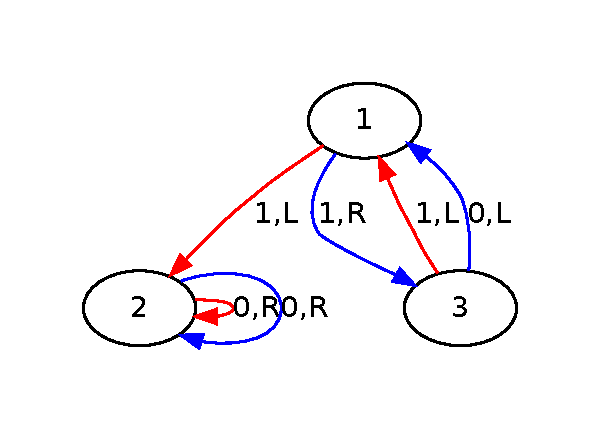
\includegraphics[width=.8\textwidth]{images/example_TM}
	\caption{State transition diagram for notional 3-state TM.}
	\label{fig:example_TM}
\end{figure}

It should be noted that all TM using this encoding assume that the 0 state is the halt state. It is not required that any TM utilize the halt state at all. The example TM above did not use the halt state. 

\subsection{Turing Machine Fitness Evaluation} 

The function of the fitness evaluation in a Genetic Algorithm is to provide the means of scoring one population candidate against another. The particular formulation that is chosen for a fitness evaluation will effect the entire outcome of any optimization. For this research, the purpose is to investigate the likelihood that an evolutionary process can produce very "complex" organisms from "simple" ones. Taken TMs as analogs for organisms, the best possible result we can hope for is a population of UTM's. So the fitness function employed must grade TMs that are most like a UTM higher than ones that are less like a UTM.  

There is not simple test for that can be applied to a TM to determine if it is in fact a UTM. If there were, you would simply apply that test to every member of a population and grade them accordingly. Lacking such a test, it is necessary to establish certain measurable qualities of a UTM that could be tested for on a candidate. The fundamental problem with this approach is that when a specific candidate has been shown to share a lot of the qualities that you have associated with a UTM, there is no single logical path that can extend that information to show that the candidate is actually a UTM (that's why there is no test!). 

Instead of testing directly for qualities of candidate TMs that are similar to those of a UTM, a more simple fitness evaluation was used, which follows more directly with the stated hypothesis. TMs are scored based on the complexity of their output. This complexity is measured by applying a compression algorithm to the output string of the turing machine, and then using the resulting size of the compressed data as the fitness of the TM. The DEFLATE compression algorithm was selected because it is a lossless compression algorithm and is part of the ruby standard library.

Since the output of a TM is dependent on the input given to it, the outcome of this fitness evaluation is highly dependent on the input given to each candidate TM as well. Three interesting input types were evaluated: 

\begin{enumerate}
	\item Fixed input string for all generations
	\item Randomly generated input string for each generation
	\item Input string with some mutation between generations
\end{enumerate}

The first option tests the outcome of an optimization where each generation is being given effectively the same exact test as all the others. TMs which are good at making complex output for this specific input will thrive. The second option basically generated a random new test for each generation, and only TMs that can produce complex output for arbitrary input will thrive. These TMs could be considered very adaptable. The third option presents a hybrid approach to the previous two; here each successive generation is operating on an input string which is similar to the last (how similar depends on the mutation rate) but not idendtical. Over a large number of generations however the input string is effectively appears random. For this research, the when using the third input string option, a mutation rate of 50\% was used. 

\subsection{Results Visualization}

The results visualization system provides a graphical summary of the progression of an optimziation. It was written using Ruby On Rails and takes advantage of two graphical plotting tools: gcharts and graphviz.
